\section{Team Members and Workloads}

The project is developed by \textbf{Group LHPD2}, consisting of the following members:

\begin{center}
    \renewcommand{\arraystretch}{1.5}
    \begin{tabularx}{\textwidth}{||c|c|c|X||}
    \hline
    \textbf{No.} & \textbf{Full Name} & \textbf{Student ID} & \textbf{Task Assigned} \\
    \hline
    1 & Nguyen Quang Phu & 2252621 & Team leader; Repository management; Participate and Ensure everything stays on schedule and verify all work done by other members. \\
    \hline
    2 & Pham Huynh Bao Dai & 2252139 & Data preparation; Data preprocessing; feature engineering; Visualization; Document Data Collecting; Preprocessing and Merging. \\
    \hline
    3 & Nguyen Thanh Dat & 2252145 & Model training and evaluating; Model implementation (Decision Tree, Random Forest, XGBoost, Perceptron - ANN, MLP); Document Model Implementation.  \\
    \hline
    4 & Nguyen Tien Hung & 2252280 & Model training and evaluating; Model implementation (GA, HMM Bayesian Network, Logistic Regression, LSTM); Document Model Implementation. \\
    \hline
    5 & Nguyen Thien Loc & 2252460 & Visualization; Model evaluation; hyperparameter tuning; Model Comparison; Document Performance analysis.  \\
    \hline
    \end{tabularx}
\end{center} 

\section{Project Organization and Requirements}

The project follows structured collaboration and engineering practices, adhering to the following guidelines:

\subsection{Team Collaboration and Version Control}

\begin{itemize}
    \item Each member actively contributes to the repository, ensuring distributed workload and participation.
    \item The main repository is hosted on GitHub at:  
    \textbf{\url{https://github.com/pdz1804/ML_LHPD2}}.
    \item The submitted README file is stored in the repository at: \url{https://github.com/pdz1804/ML_LHPD2/blob/main/notebooks/assignment1/ML_LHPD2_Ass1_README.md}
    \item The team's report for Assignment 1 is located in: \url{https://github.com/pdz1804/ML_LHPD2/tree/main/reports/final_project/}
    \item The repository follows a branching strategy, where each member develops on a dedicated branch and submits changes via pull requests.
    \item Code reviews and discussions are conducted to ensure quality, maintainability, and adherence to best practices.
    \item Version control best practices are maintained, with regular commits, documentation, and codebase integrity.
\end{itemize}

\subsection{GitHub Repository Structure}

The repository is structured to support multiple problem formulations, model implementations, and comparative analyses while maintaining a clean code structure and proper documentation.

\begin{itemize}
    \item \textbf{Main repository}: Created and maintained by a designated team member.
    \item \textbf{Forking workflow}: Other members fork and contribute via pull requests.
    \item \textbf{Branching strategy}: Different branches are created for models and features to ensure isolated development.
    \item \textbf{Comprehensive documentation}: Ensures clarity in problem definitions, methodologies, and results.
\end{itemize}

\subsection{Key Requirements}

\begin{itemize}
    \item \textbf{Clear problem documentation}: Problem statements and their variations are well-documented.
    \item \textbf{Consistent implementation interface}: All models follow a standardized interface to ensure ease of comparison.
    \item \textbf{Comprehensive testing}: Each component undergoes rigorous testing.
    \item \textbf{Detailed comparative analysis}: Models are evaluated across multiple performance metrics.
    \item \textbf{Regular code reviews and pull requests}: Maintains code integrity and quality.
    \item \textbf{Version control best practices}: Ensures organized and maintainable development.
\end{itemize}

\section{Repository Structure}

To facilitate maintainability, scalability, and efficient collaboration, the repository follows a structured layout:

\begin{figure}[H]
    \centering
    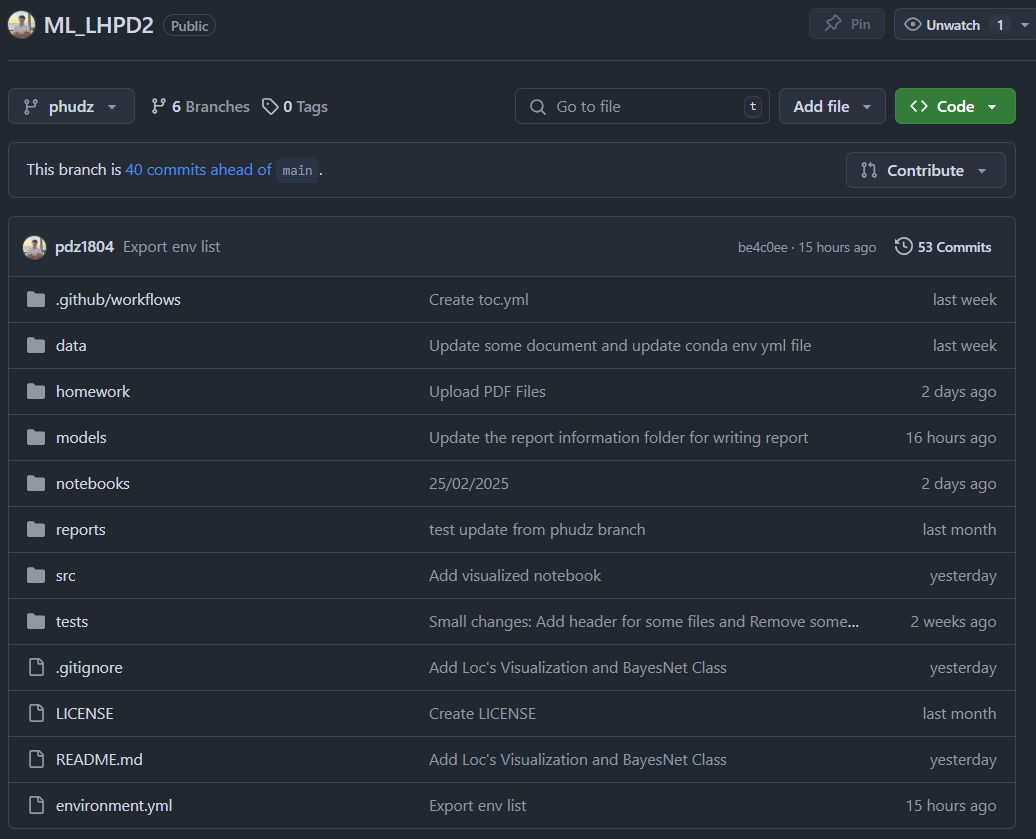
\includegraphics[width=0.75\textwidth]{img/progress/github_repo.PNG}
    \caption{Github Repository Structure}
    \label{fig:github-repo}
\end{figure}

\subsection{How to Run This Project}

\subsubsection{Clone the Repository}

\begin{lstlisting}[language=bash]
git clone https://github.com/pdz1804/ML_LHPD2
cd ML_LHPD2
\end{lstlisting}

\subsubsection{Environment Setup}

To train the model locally, install dependencies using the provided \texttt{environment.yml} file. Ensure Conda is installed first.

\begin{lstlisting}[language=bash]
conda env create -f environment.yml
conda activate ml_env  # Replace ml_env with your environment name
\end{lstlisting}

\subsection{Project Exploration}

The project structure contains several key components:

\begin{itemize}
    \item \textbf{Data Collection:} To know how we collected all the data, visit the \texttt{data} folder.
    \item \textbf{Final Preprocessed Dataset:} The final preprocessed dataset can be found at this link: 
    \href{https://www.kaggle.com/datasets/zphudzz/tweets-clean-posneg-v1}{Tweets Clean PosNeg v1}.
    \item \textbf{Preprocessing:} To learn how we preprocess, make all datasets consistent to merge:
    \begin{itemize}
        \item Notebook: \texttt{src/data/process.ipynb}
        \item Utility file: \texttt{src/data/preprocess.py}
    \end{itemize}
    \item \textbf{Feature Engineering:} To know how we create features, visit:
    \begin{itemize}
        \item Utility file: \texttt{src/features/build\_features\_utils.py}
    \end{itemize}
    \item \textbf{Model Training and Evaluation:} To understand hyperparameter tuning, k-fold cross-validation, and model training:
    \begin{itemize}
        \item Hyperparameter tuning utility: \texttt{src/models/models\_utils.py}
        \item Training notebook: \texttt{src/models/train\_model.ipynb}
    \end{itemize}
    \item \textbf{Visualization Functions:} We have created visualization functions in the folder:
    \begin{itemize}
        \item Location: \texttt{src/visualization/}
    \end{itemize}
    Although these functions are not currently used in code (as we rely on inline plotting), they will be utilized in Assignment 2.
    \item \textbf{Dependencies:} The file \texttt{environment.yml} contains details about libraries or dependencies required for executing this project.
\end{itemize}

\newpage
